\documentclass{report}
\usepackage{graphicx} % Required for inserting images
\usepackage[a4paper, total={6in, 9in}]{geometry}
\usepackage{amsmath}
\usepackage{enumitem}
% \usepackage{minted}
\usepackage{hyperref}
\hypersetup{
    colorlinks=true,
    linkcolor=blue,
    filecolor=magenta,      
    urlcolor=cyan,
    pdftitle={Fast Fourier transform}
    }

\begin{document}

% \maketitle
\begin{titlepage}
    \centering
    \vspace*{2cm}
    
\includegraphics[width=0.25\textwidth]{buet.png}\\
    \vspace{1.5cm}
    {\Large \textbf{Bangladesh University of Engineering and Technology} \par}
    \vspace{2cm}
    {\LARGE \textbf{CSE 300} \par}
    \vspace{1cm}
    {\Large Report on \par}
    \vspace{0.5cm}
    {\LARGE \textbf{Fast Fourier Transform (FFT):\\[0.5em] A Revolutionizing Algorithm} \par}
    \vspace{1.5cm}
    {\large \textbf{Authors:} \par}
    \vspace{0.5cm}
    {\large Tanvirul Islam Turad (2005011) \par}
    {\large Tanvir Hossain (2005014) \par}
    {\large MD. Jakaria Hossain\par}
    \vspace{2cm}
    {\large Date: \today \par}
\end{titlepage}

\tableofcontents

\newpage
\chapter{Applications}
FFT is the core component of frequency domain analysis, also known as spectrum analysis, in signal processing. It is widely used in data compression, spectral estimation, signal filtering, and other applications. Analysis in both the frequency and time domains can be done simultaneously using FFT variations like the short-time Fourier transform. These methods can be applied to a wide range of signals, including communication, radar, audio and speech, and other sensor data signals. Additionally, FFT is occasionally employed as a transitional step before more sophisticated signal processing methods. FFT is used for filtering and picture compression in image processing. In mathematics and physics, partial differential equations (PDEs) are also solved using FFT.
\section{FFT in signal processing}
FFT is most frequently used to convert signals from the time domain to the frequency domain.
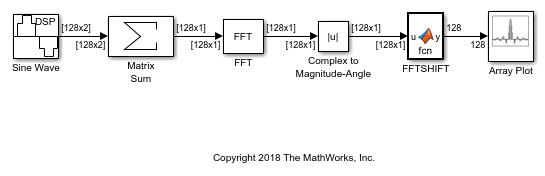
\includegraphics[scale=0.8]{t_f_dom.png}
The fundamental algorithm used for time-frequency based signal analysis in many simulation programs, such as MATLAB, is FFT. The FFT algorithm was utilized by MATLAB's Signal Processing $Toolbox^{TM}$ to display spectograms and persistent spectrums, which are time-frequency views that display the proportion of a signal's duration that a certain frequency is present.\\
\begin{tabular}{c c}
    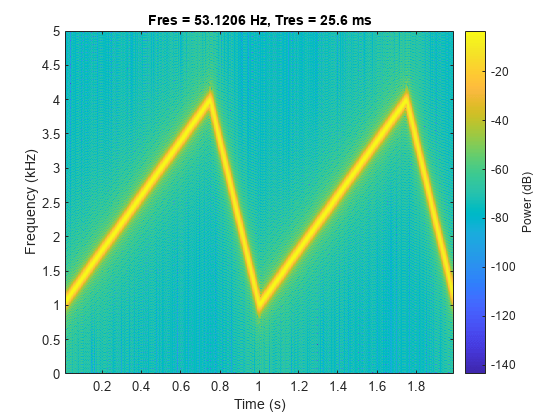
\includegraphics[scale=0.35]{signal_1.png}    &  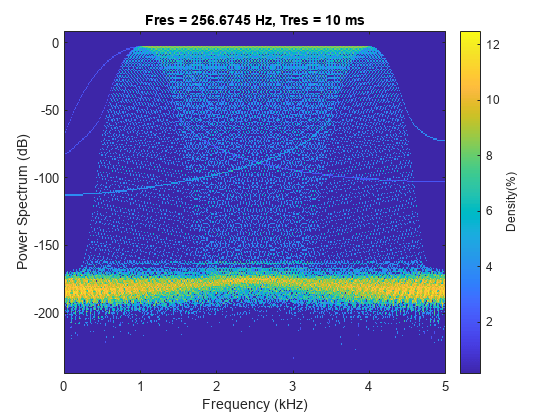
\includegraphics[scale=0.35]{signal_2.png}
    \end{tabular}
FFT helps in radar signal analysis, target detection, and tracking. FFT aids in underwater acoustics, target detection, and classification. 
\section{FFT in Communications}
    \begin{itemize}[]
            \item Digital communication systems: FFT is utilized in modulation and demodulation schemes such as OFDM (Orthogonal Frequency Division Multiplexing) used in Wi-Fi, LTE, and digital television.
            \item Channel estimation and equalization: FFT helps in estimating the channel characteristics and compensating for distortions in communication channels.
    \end{itemize}
\section{FFT in Instrumentation}
\begin{itemize}[]
            \item Spectrum analysis: FFT is employed in spectrum analyzers for measuring frequency components of signals.
            \item Biomedical signal analysis: FFT is used in the analysis of EEG (Electroencephalography), ECG (Electrocardiography), and other biomedical signals for diagnosis and monitoring.
        \end{itemize}
\section{FFT in Control Systems}
    \begin{itemize}[]
            \item Control system analysis: FFT is used in identifying system dynamics, frequency response analysis, and stability analysis.
            \item Control system design: FFT helps in designing controllers and compensators for systems with frequency-dependent characteristics.
    \end{itemize}
\section{FFT in Geophysics and Seismology}
    \begin{itemize}[]
        \item Earthquake analysis: FFT is used in seismic data processing for earthquake detection, location, and magnitude estimation.\\
        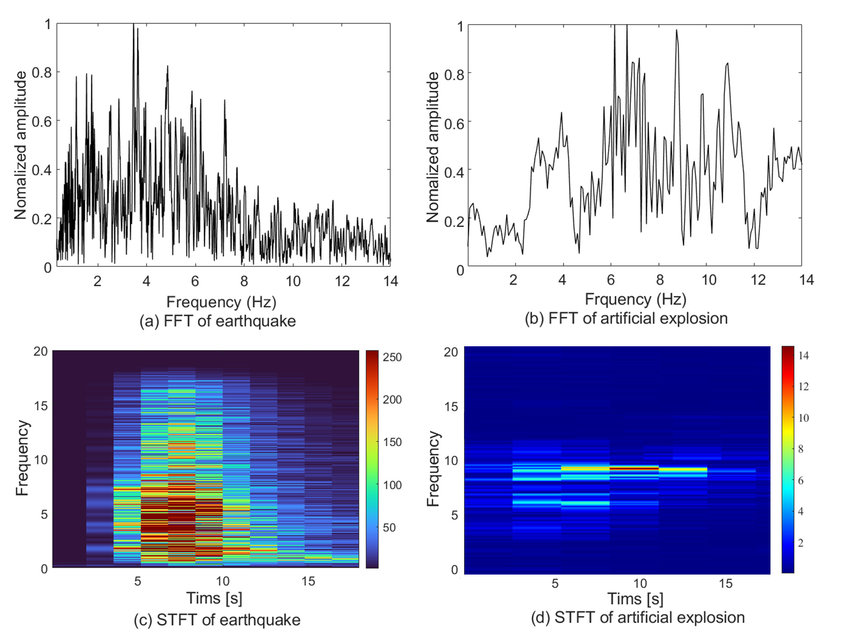
\includegraphics[scale=0.5]{seismic_signal_1.jpg}
        \item Exploration geophysics: FFT assists in the interpretation of seismic data for oil and gas exploration.
    \end{itemize}
\section{FFT in Medical Imaging}
    \begin{itemize}[]
        \item MRI (Magnetic Resonance Imaging): FFT is utilized in MRI for image reconstruction from raw data acquired during scans.
        \item CT (Computed Tomography): FFT is used in image reconstruction algorithms to convert raw projection data into cross-sectional images.
    \end{itemize}
\section{FFT in Astrophysics and Cosmology}
    \begin{itemize}[]
        \item Radio astronomy: FFT is employed in processing radio signals received from celestial objects for analysis and imaging.
        \item Cosmology: FFT assists in analyzing cosmic microwave background radiation data for studying the early universe.
    \end{itemize}
\section{FFT in Computer Science}
DFT, a special variation of FFT can be used in a huge variety of other problems, which at the first glance have nothing to do with multiplying polynomials.

\subsection{All possible sums}

We are given two arrays $a[]$ and $b[]$. We have to find all possible sums $a[i] + b[j]$, and for each sum count how often it appears.

For example for $a = [1,~ 2,~ 3]$ and $b = [2,~ 4]$ we get: then sum $3$ can be obtained in $1$ way, the sum $4$ also in $1$ way, $5$ in $2$, $6$ in $1$, $7$ in $1$.

We construct for the arrays $a$ and $b$ two polynomials $A$ and $B$. The numbers of the array will act as the exponents in the polynomial ($a[i] \Rightarrow x^{a[i]}$); and the coefficients of this term will be how often the number appears in the array.

Then, by multiplying these two polynomials in $O(n \log n)$ time, we get a polynomial $C$, where the exponents will tell us which sums can be obtained, and the coefficients tell us how often. To demonstrate this on the example:
$$(1 x^1 + 1 x^2 + 1 x^3) (1 x^2 + 1 x^4) = 1 x^3 + 1 x^4 + 2 x^5 + 1 x^6 + 1 x^7$$

\subsection{All possible scalar products}

We are given two arrays $a[]$ and $b[]$ of length $n$. We have to compute the products of $a$ with every cyclic shift of $b$.

We generate two new arrays of size $2n$: We reverse $a$ and append $n$ zeros to it. And we just append $b$ to itself. When we multiply these two arrays as polynomials, and look at the coefficients $c[n-1],~ c[n],~ \dots,~ c[2n-2]$ of the product $c$, we get:
$$c[k] = \sum_{i+j=k} a[i] b[j]$$

And since all the elements $a[i] = 0$ for $i \ge n$:
$$c[k] = \sum_{i=0}^{n-1} a[i] b[k-i]$$

It is easy to see that this sum is just the scalar product of the vector $a$ with the $(k - (n - 1))$-th cyclic left shift of $b$. Thus these coefficients are the answer to the problem, and we were still able to obtain it in $O(n \log n)$ time. Note here that $c[2n-1]$ also gives us the $n$-th cyclic shift but that is the same as the $0$-th cyclic shift so we don't need to consider that separately into our answer.

\subsection{Two stripes}

We are given two Boolean stripes (cyclic arrays of values $0$ and $1$) $a$ and $b$. We want to find all ways to attach the first stripe to the second one, such that at no position we have a $1$ of the first stripe next to a $1$ of the second stripe.

The problem doesn't actually differ much from the previous problem. Attaching two stripes just means that we perform a cyclic shift on the second array, and we can attach the two stripes, if scalar product of the two arrays is $0$.

\subsection{String matching}

We are given two strings, a text $T$ and a pattern $P$, consisting of lowercase letters. We have to compute all the occurrences of the pattern in the text.

We create a polynomial for each string ($T[i]$ and $P[I]$ are numbers between $0$ and $25$ corresponding to the $26$ letters of the alphabet):
$$A(x) = a_0 x^0 + a_1 x^1 + \dots + a_{n-1} x^{n-1}, \quad n = |T|$$

with
$$a_i = \cos(\alpha_i) + i \sin(\alpha_i), \quad \alpha_i = \frac{2 \pi T[i]}{26}.$$

And
$$B(x) = b_0 x^0 + b_1 x^1 + \dots + b_{m-1} x^{m-1}, \quad m = |P|$$

with
$$b_i = \cos(\beta_i) - i \sin(\beta_i), \quad \beta_i = \frac{2 \pi P[m-i-1]}{26}.$$

Notice that with the expression $P[m-i-1]$ explicitly reverses the pattern.

The $(m-1+i)$th coefficients of the product of the two polynomials $C(x) = A(x) \cdot B(x)$ will tell us, if the pattern appears in the text at position $i$.
$$c_{m-1+i} = \sum_{j = 0}^{m-1} a_{i+j} \cdot b_{m-1-j} = \sum_{j=0}^{m-1} \left(\cos(\alpha_{i+j}) + i \sin(\alpha_{i+j})\right) \cdot \left(\cos(\beta_j) - i \sin(\beta_j)\right)$$

with $\alpha_{i+j} = \frac{2 \pi T[i+j]}{26}$ and $\beta_j = \frac{2 \pi P[j]}{26}$

If there is a match, than $T[i+j] = P[j]$, and therefore $\alpha_{i+j} = \beta_j$. This gives (using the Pythagorean trigonometric identity):
\[\begin{align} c_{m-1+i} &= \sum_{j = 0}^{m-1} \left(\cos(\alpha_{i+j}) + i \sin(\alpha_{i+j})\right) \cdot \left(\cos(\alpha_{i+j}) - i \sin(\alpha_{i+j})\right) \\ &= \sum_{j = 0}^{m-1} \cos(\alpha_{i+j})^2 + \sin(\alpha_{i+j})^2 = \sum_{j = 0}^{m-1} 1 = m \end{align}\]

If there isn't a match, then at least a character is different, which leads that one of the products $a_{i+1} \cdot b_{m-1-j}$ is not equal to $1$, which leads to the coefficient $c_{m-1+i} \ne m$.

\subsection{String matching with wildcards}

This is an extension of the previous problem. This time we allow that the pattern contains the wildcard character $\*$, which can match every possible letter. E.g. the pattern $a*c$ appears in the text $abccaacc$ at exactly three positions, at index $0$, index $4$ and index $5$.

We create the exact same polynomials, except that we set $b_i = 0$ if $P[m-i-1] = *$. If $x$ is the number of wildcards in $P$, then we will have a match of $P$ in $T$ at index $i$ if $c_{m-1+i} = m - x$.

% \newpage

\subsection*{More problems to explore}


\href{https://www.spoj.com/problems/POLYMUL/}{POLYMUL - Polynomial Multiplication}

\href{https://www.spoj.com/problems/MAXMATCH/}{MAXMATCH - Maximum Self-Matching}

\href{https://www.spoj.com/problems/ADAMATCH/}{ADAMATCH - Ada and Nucleobase}

\href{https://codeforces.com/problemset/problem/954/I}{Yet Another String Matching Problem}

\href{https://codeforces.com/problemset/problem/958/F3}{Lightsabers (hard)}

\href{https://codeforces.com/contest/1398/problem/G}{Running Competition}

\href{https://codeforces.com/contest/754/problem/E}{Dasha and cyclic table}

\href{https://codeforces.com/problemset/problem/1667/E}{Centroid Probabilities}

\href{https://www.codechef.com/COOK112A/problems/MMNN01}{Expected Number of Customer}

\href{https://www.codechef.com/SEPT19A/problems/PSUM}{Power Sum}

\href{https://open.kattis.com/problems/aplusb}{A+B Problem}

\href{https://open.kattis.com/problems/kinversions}{K-Inversions}

\chapter{Conclusion}

In conclusion, the Fast Fourier Transform (FFT) technique is a cornerstone in signal processing and beyond. Its extraordinary efficiency in computing the Discrete Fourier Transform (DFT) has enabled advances in a wide range of applications.

Throughout this report, we have explored the diverse applications of the FFT algorithm, spanning signal processing, communications, instrumentation, control systems, geophysics, medical imaging, finance, astrophysics, and cosmology. From audio and image processing to radar and sonar signal analysis, from medical diagnostics to seismic data interpretation, the FFT algorithm finds itself at the heart of countless innovative solutions.

The versatility of the FFT algorithm supports vital technologies like digital communication networks, medical imaging equipment, and astronomical observatories in addition to making signal analysis and modification easier. Its widespread use highlights its significance as a vital instrument in contemporary research and engineering.

Looking ahead, as technology continues to evolve, the FFT algorithm is poised to remain an indispensable asset, enabling further breakthroughs in fields ranging from data science to space exploration. Its impact on our understanding of the world and our ability to manipulate and interpret signals is undeniable, making it a subject of continued research and application for years to come.

In essence, the FFT algorithm exemplifies the power of computational methods to unlock new insights and capabilities across a broad spectrum of disciplines, shaping the landscape of scientific inquiry and technological innovation.

\end{document}